\section{BFN fine tuning}

Before proceeding with the simulation of the overall antenna we decided to perform an optimization of the BFN.

\begin{figure}[H]
\centering
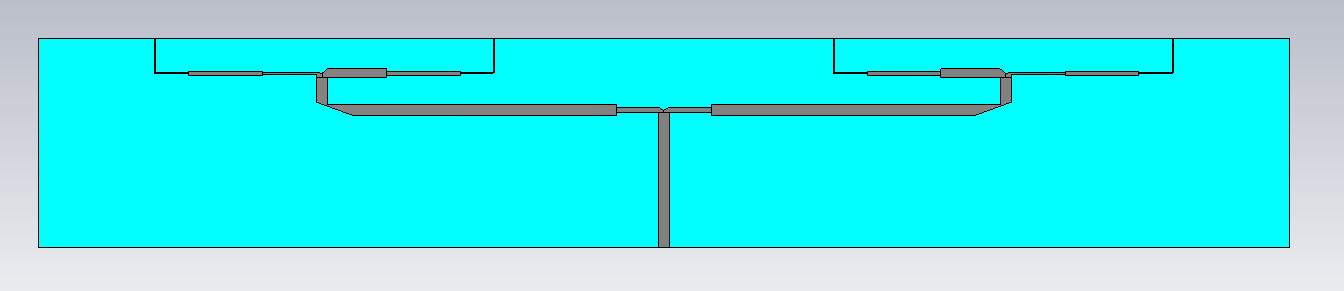
\includegraphics[scale=0.45]{BFN_look.png}
\caption{How the final BFN looks like}
\label{BFN_look}
\end{figure}

\par\medskip
\noindent
The attention was mainly focused on:

\begin{itemize}
\item tuning of the S\textsubscript{11} parameter, in order to obtain a resonant behavior at 2.45 GHz
\item achieving the best possible tapering, i.e. as close as possible to the theoretical value of 5.3 dB needed in order to get the right SLL in the final structure
\item obtaining the right phasing between the elements, i.e. phase difference as close as possible to zero, since the array must be broadside.
\end{itemize}

\par\medskip
\noindent
Before showing the results of the simulations it is worth to spend a few words about meshes; in fact, as explained in class, the correct definition of the meshgrid is fundamental in order to assure the correct behavior of the waveguide ports and a reliable analysis of all the discontinuities present inside the model. That being said, we decided to impose a refinement of the grid across the more sensitive areas (thin elements and discontinuities) and second, a symmetry plane, which allowed to reduce the simulation time thanks to the intrinsic symmetry of the structure.
\noindent
Figure \ref{BFN_mesh} gives an idea of how thin the mesh was around the critical points, while figures \ref{BFN_meshp1} and \ref{BFN_meshp2} show exactly how the settings were manipulated in order to obtain it.

\begin{figure}[H]
\centering
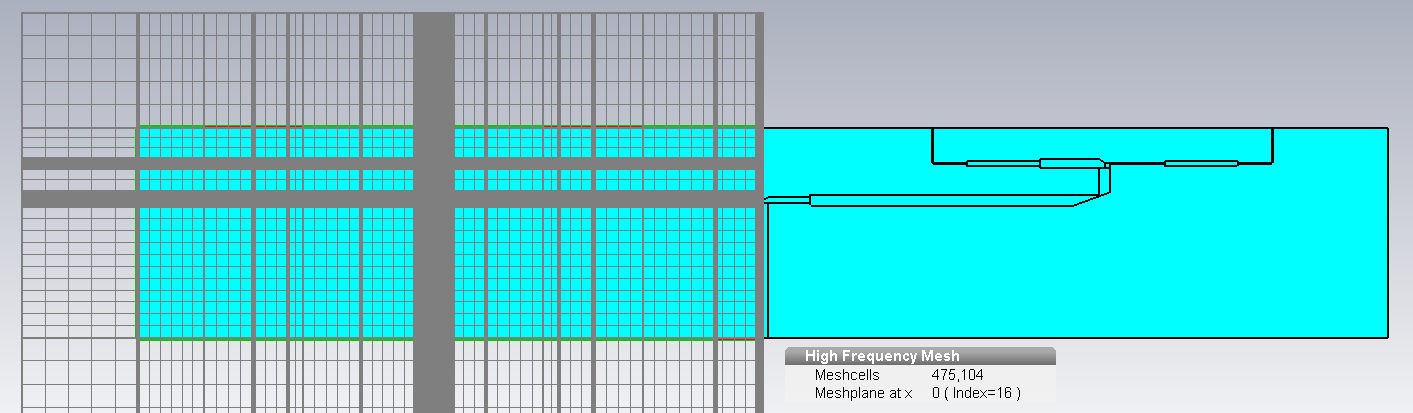
\includegraphics[scale=0.4]{BFN_mesh.png}
\caption{Mesh View of the BFN, showing the used symmetry plane setting too}
\label{BFN_mesh}
\end{figure}

\begin{figure}[H]
\centering
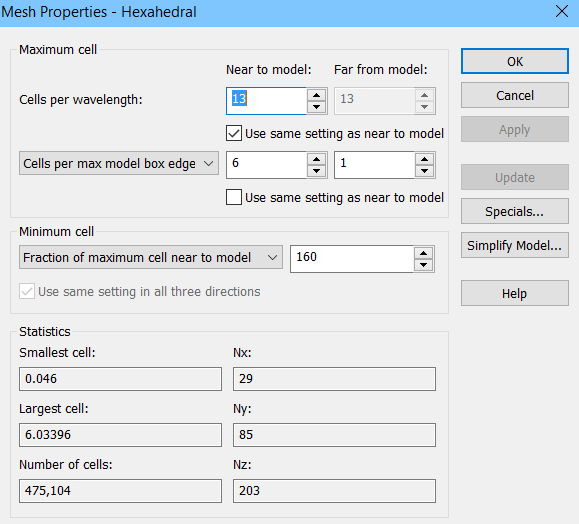
\includegraphics[scale=0.8]{BFN_meshp1.png}
\caption{Imposed Mesh Properties}
\label{BFN_meshp1}
\end{figure}

\begin{figure}[H]
\centering
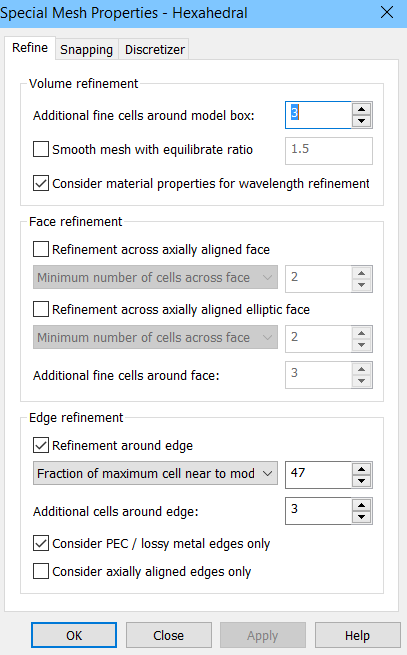
\includegraphics[scale=0.8]{BFN_meshp2.png}
\caption{Imposed Special Mesh Properties}
\label{BFN_meshp2}
\end{figure}

\par\medskip
\noindent
Now that we've concluded the discussion about adopted procedures (which obviously included a certain number of parametric sweeps and optimizer runs in order to refine the results) we can discuss the obtained parameters.

\par\medskip
\noindent
First, the S\textsubscript{11} is shown, figure \ref{BFN_S11}. The resonance point coincides almost exactly with 2.45 GHz and its level in dB is quite reassuring (-35 dB). It has to be said that we were able to obtain even lower values for our resonance (-45 dB), but in the end the shown solution was chosen because of its better behavior in terms of tapering and of the better results obtained when simulating it with the radiating elements.

\begin{figure}[H]
\centering
\includegraphics[scale=0.4]{BFN_S11.png}
\caption{S\textsubscript{11} parameter of our BFN}
\label{BFN_S11}
\end{figure}

\par\medskip
\noindent
As figures \ref{BFN_tapering} and \ref{BFN_phase} show, the tapering is around 5.05 dB while the phase difference between adjacent elements is lower than 1\textsuperscript{$\circ$}.

\begin{figure}[H]
\centering
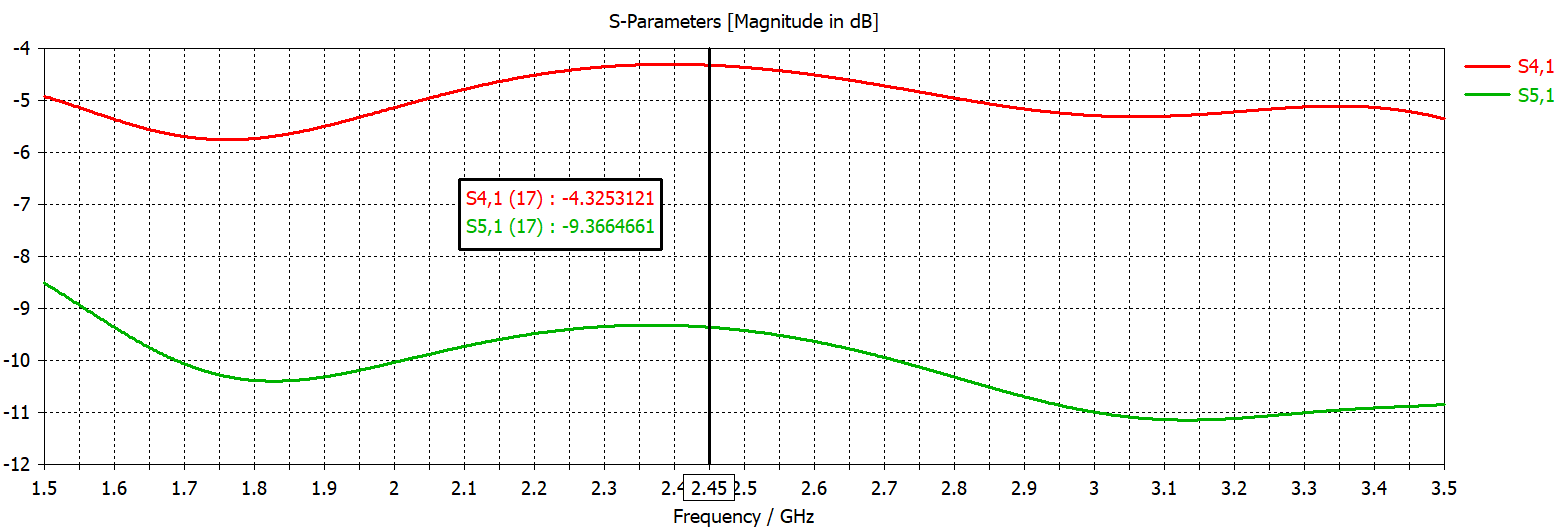
\includegraphics[scale=0.4]{BFN_tapering.png}
\caption{behavior in terms of tapering}
\label{BFN_tapering}
\end{figure}

\begin{figure}[H]
\centering
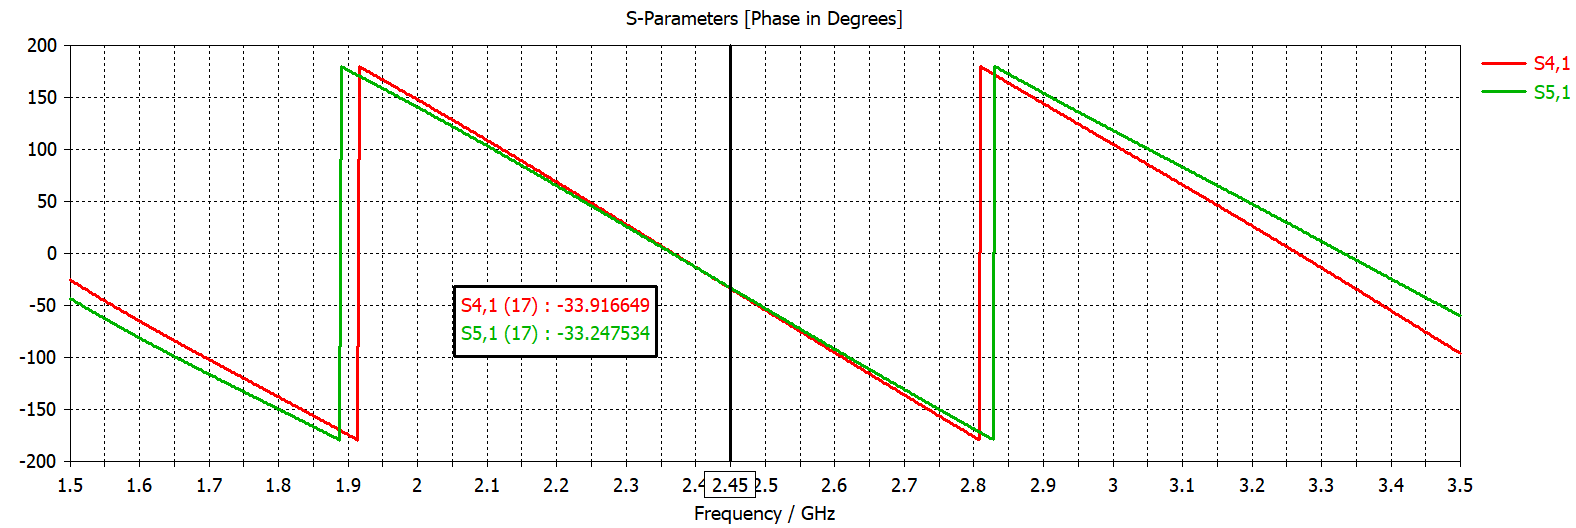
\includegraphics[scale=0.4]{BFN_phase.png}
\caption{behavior in terms of phase}
\label{BFN_phase}
\end{figure}

\par\medskip
\noindent
Last but not least, figure \ref{BFN_bands} shows an estimation of the -10 and -20 dB obtained bandwidths.

\begin{figure}[H]
\centering
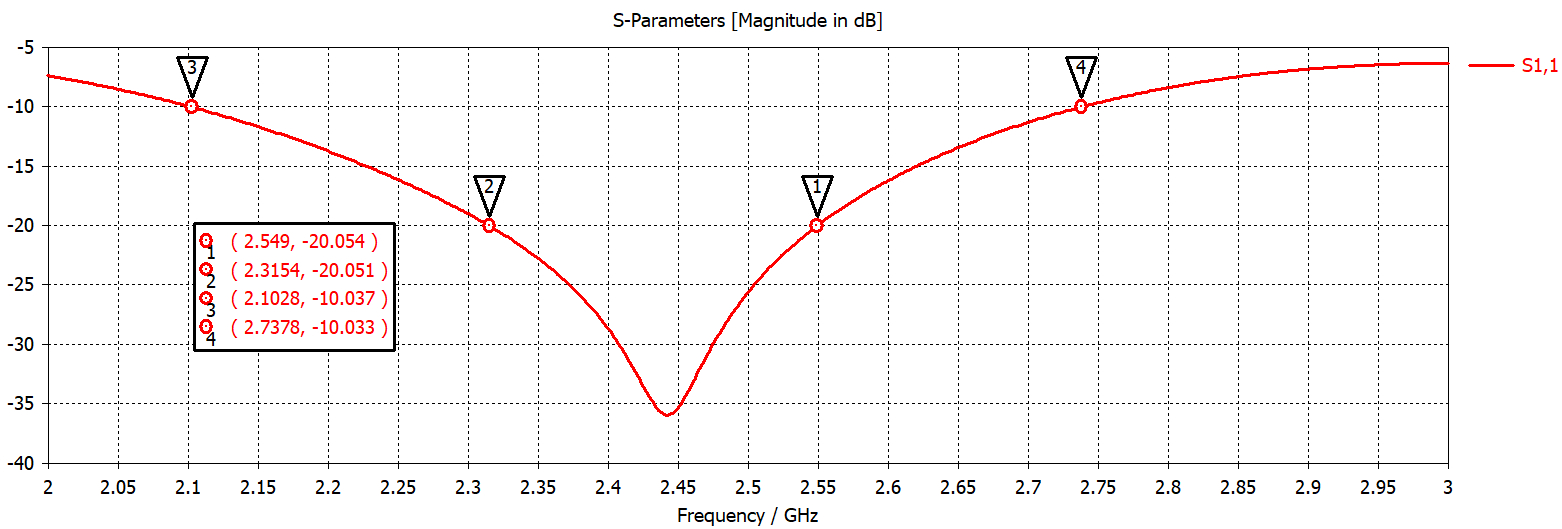
\includegraphics[scale=0.4]{BFN_bands.png}
\caption{estimation of the bandwidth of the BFN}
\label{BFN_bands}
\end{figure}
